\begin{figure*}[!ht]
    \centering
    \begin{subfigure}[t]{0.3\textwidth}
        \centering
        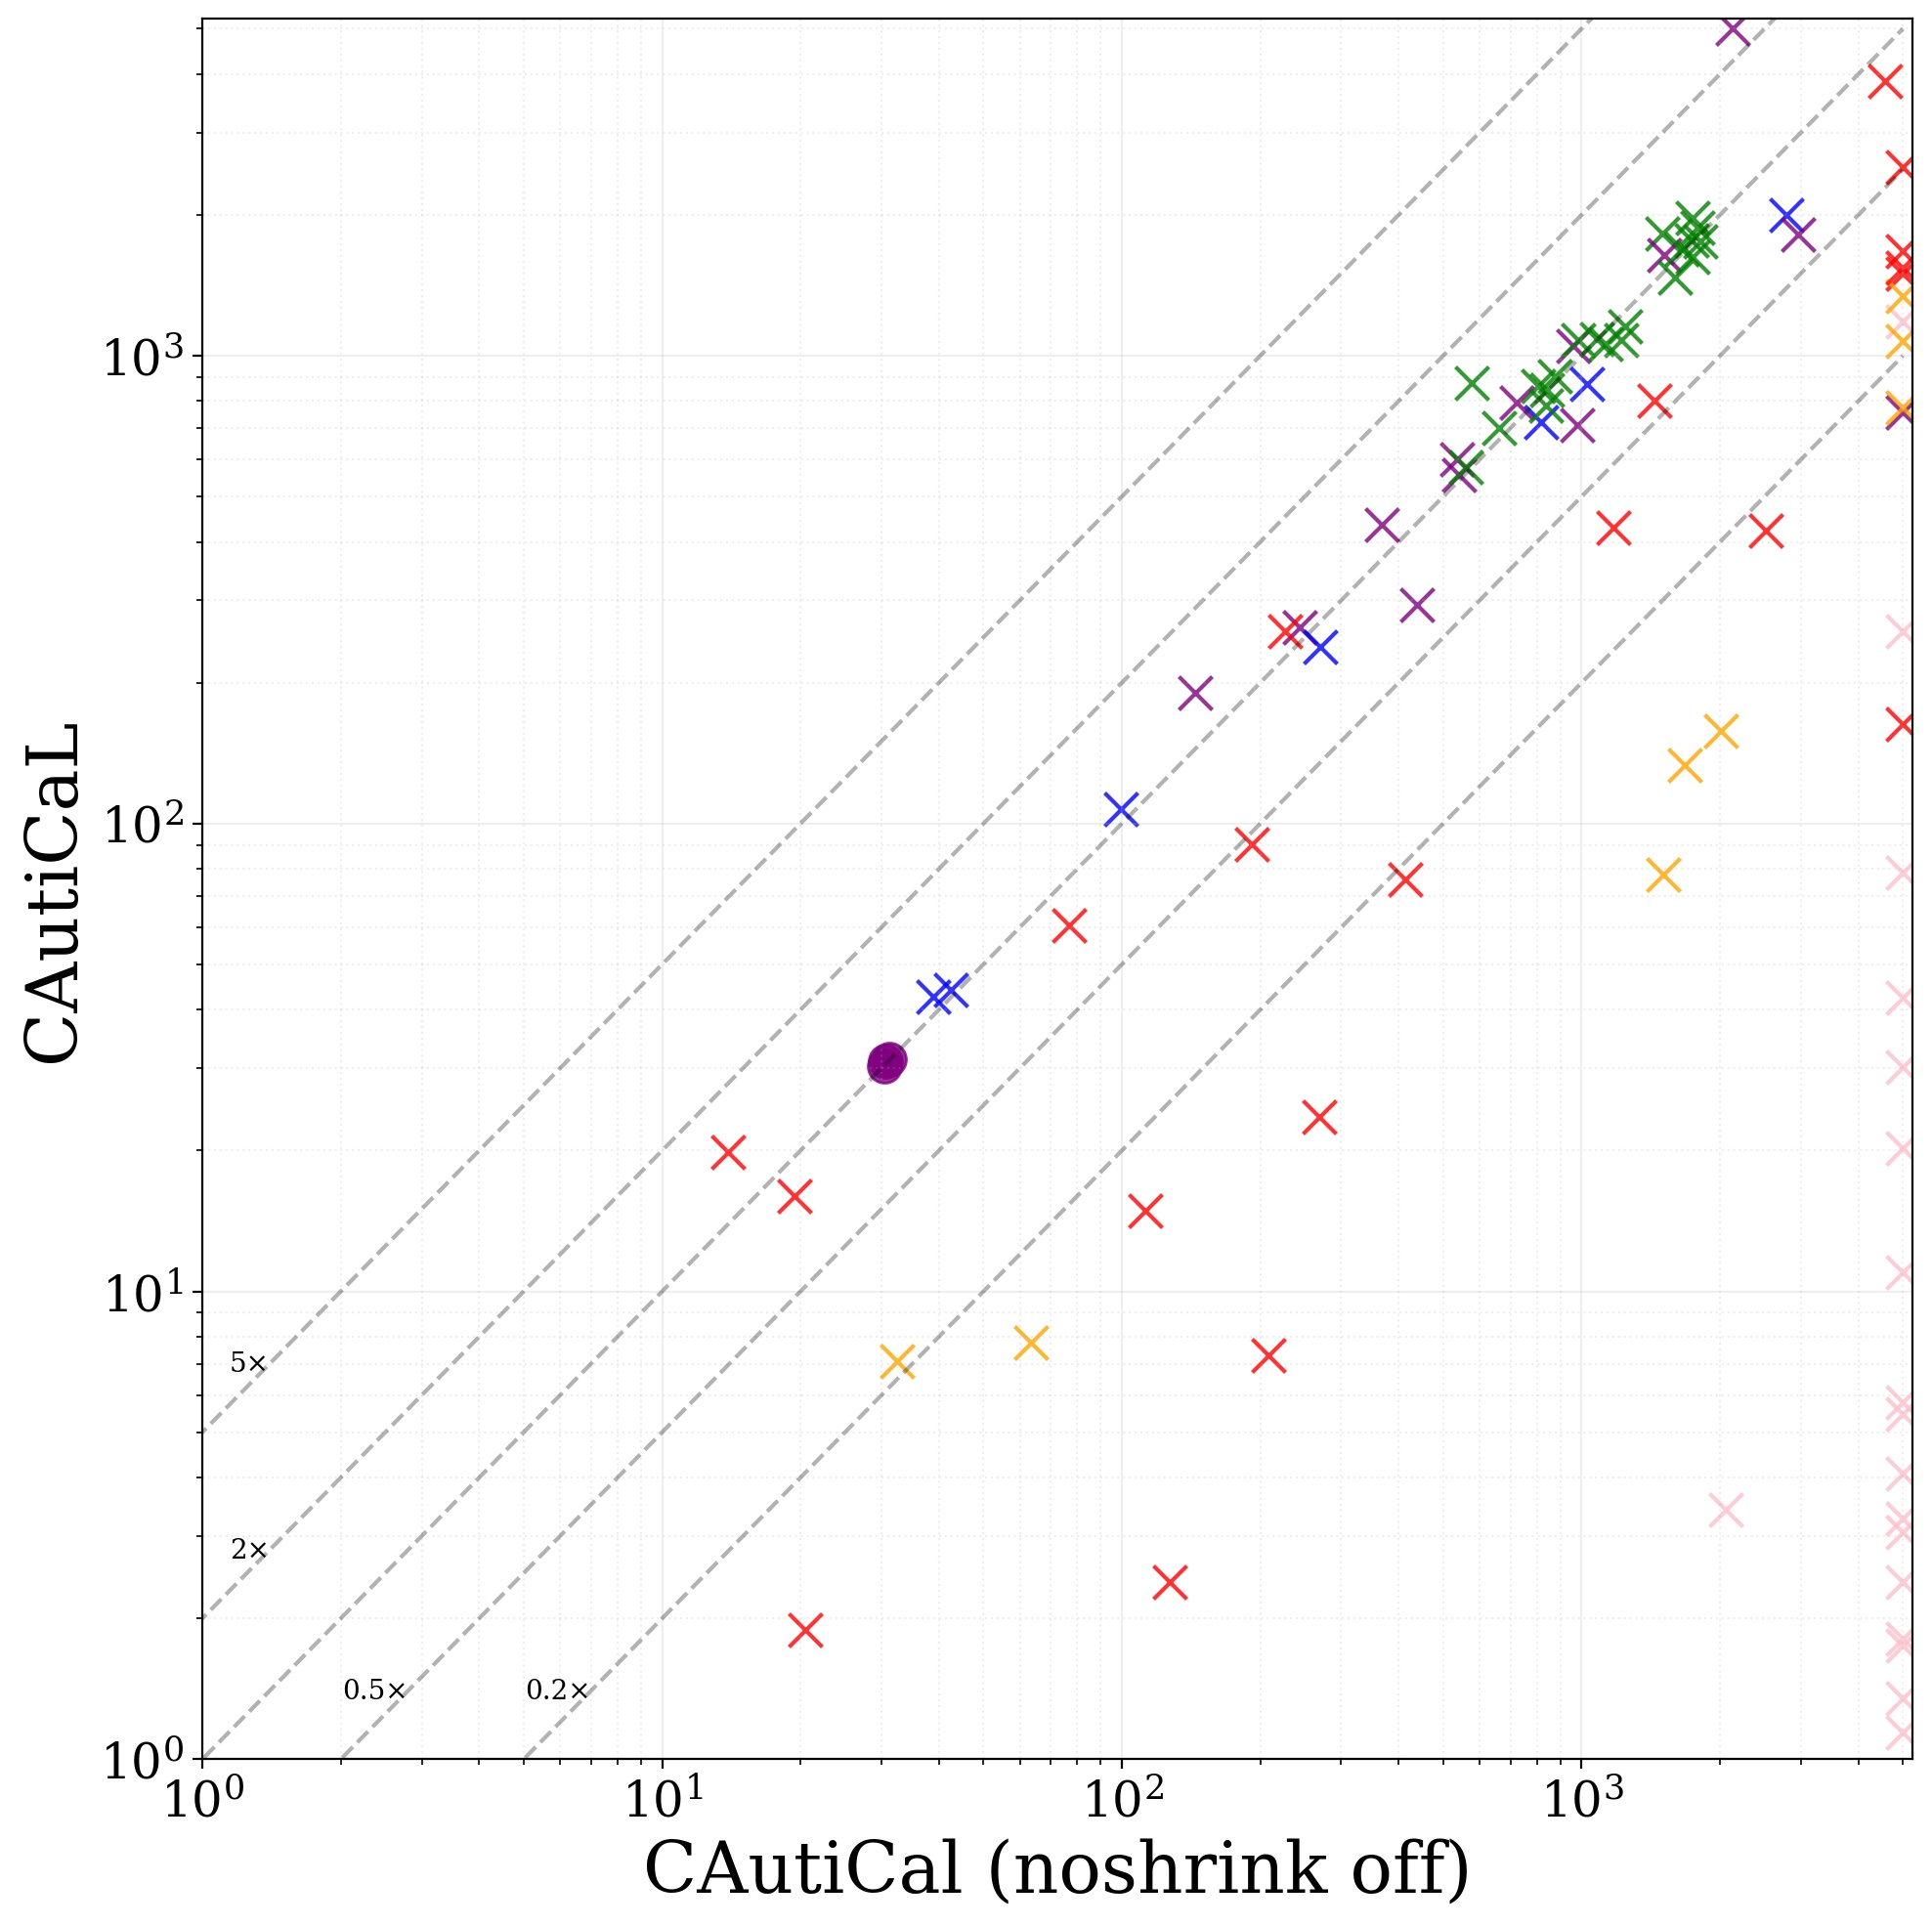
\includegraphics[width=\textwidth]{figs/globalnoshrink_heuristic_comparison.jpg}
        \caption{\tool compared to \tool with \textsf{shrink} turned off}
        \label{fig:global-no-shrink}
    \end{subfigure}
    \hfill
    \begin{subfigure}[t]{0.3\textwidth}
        \centering
        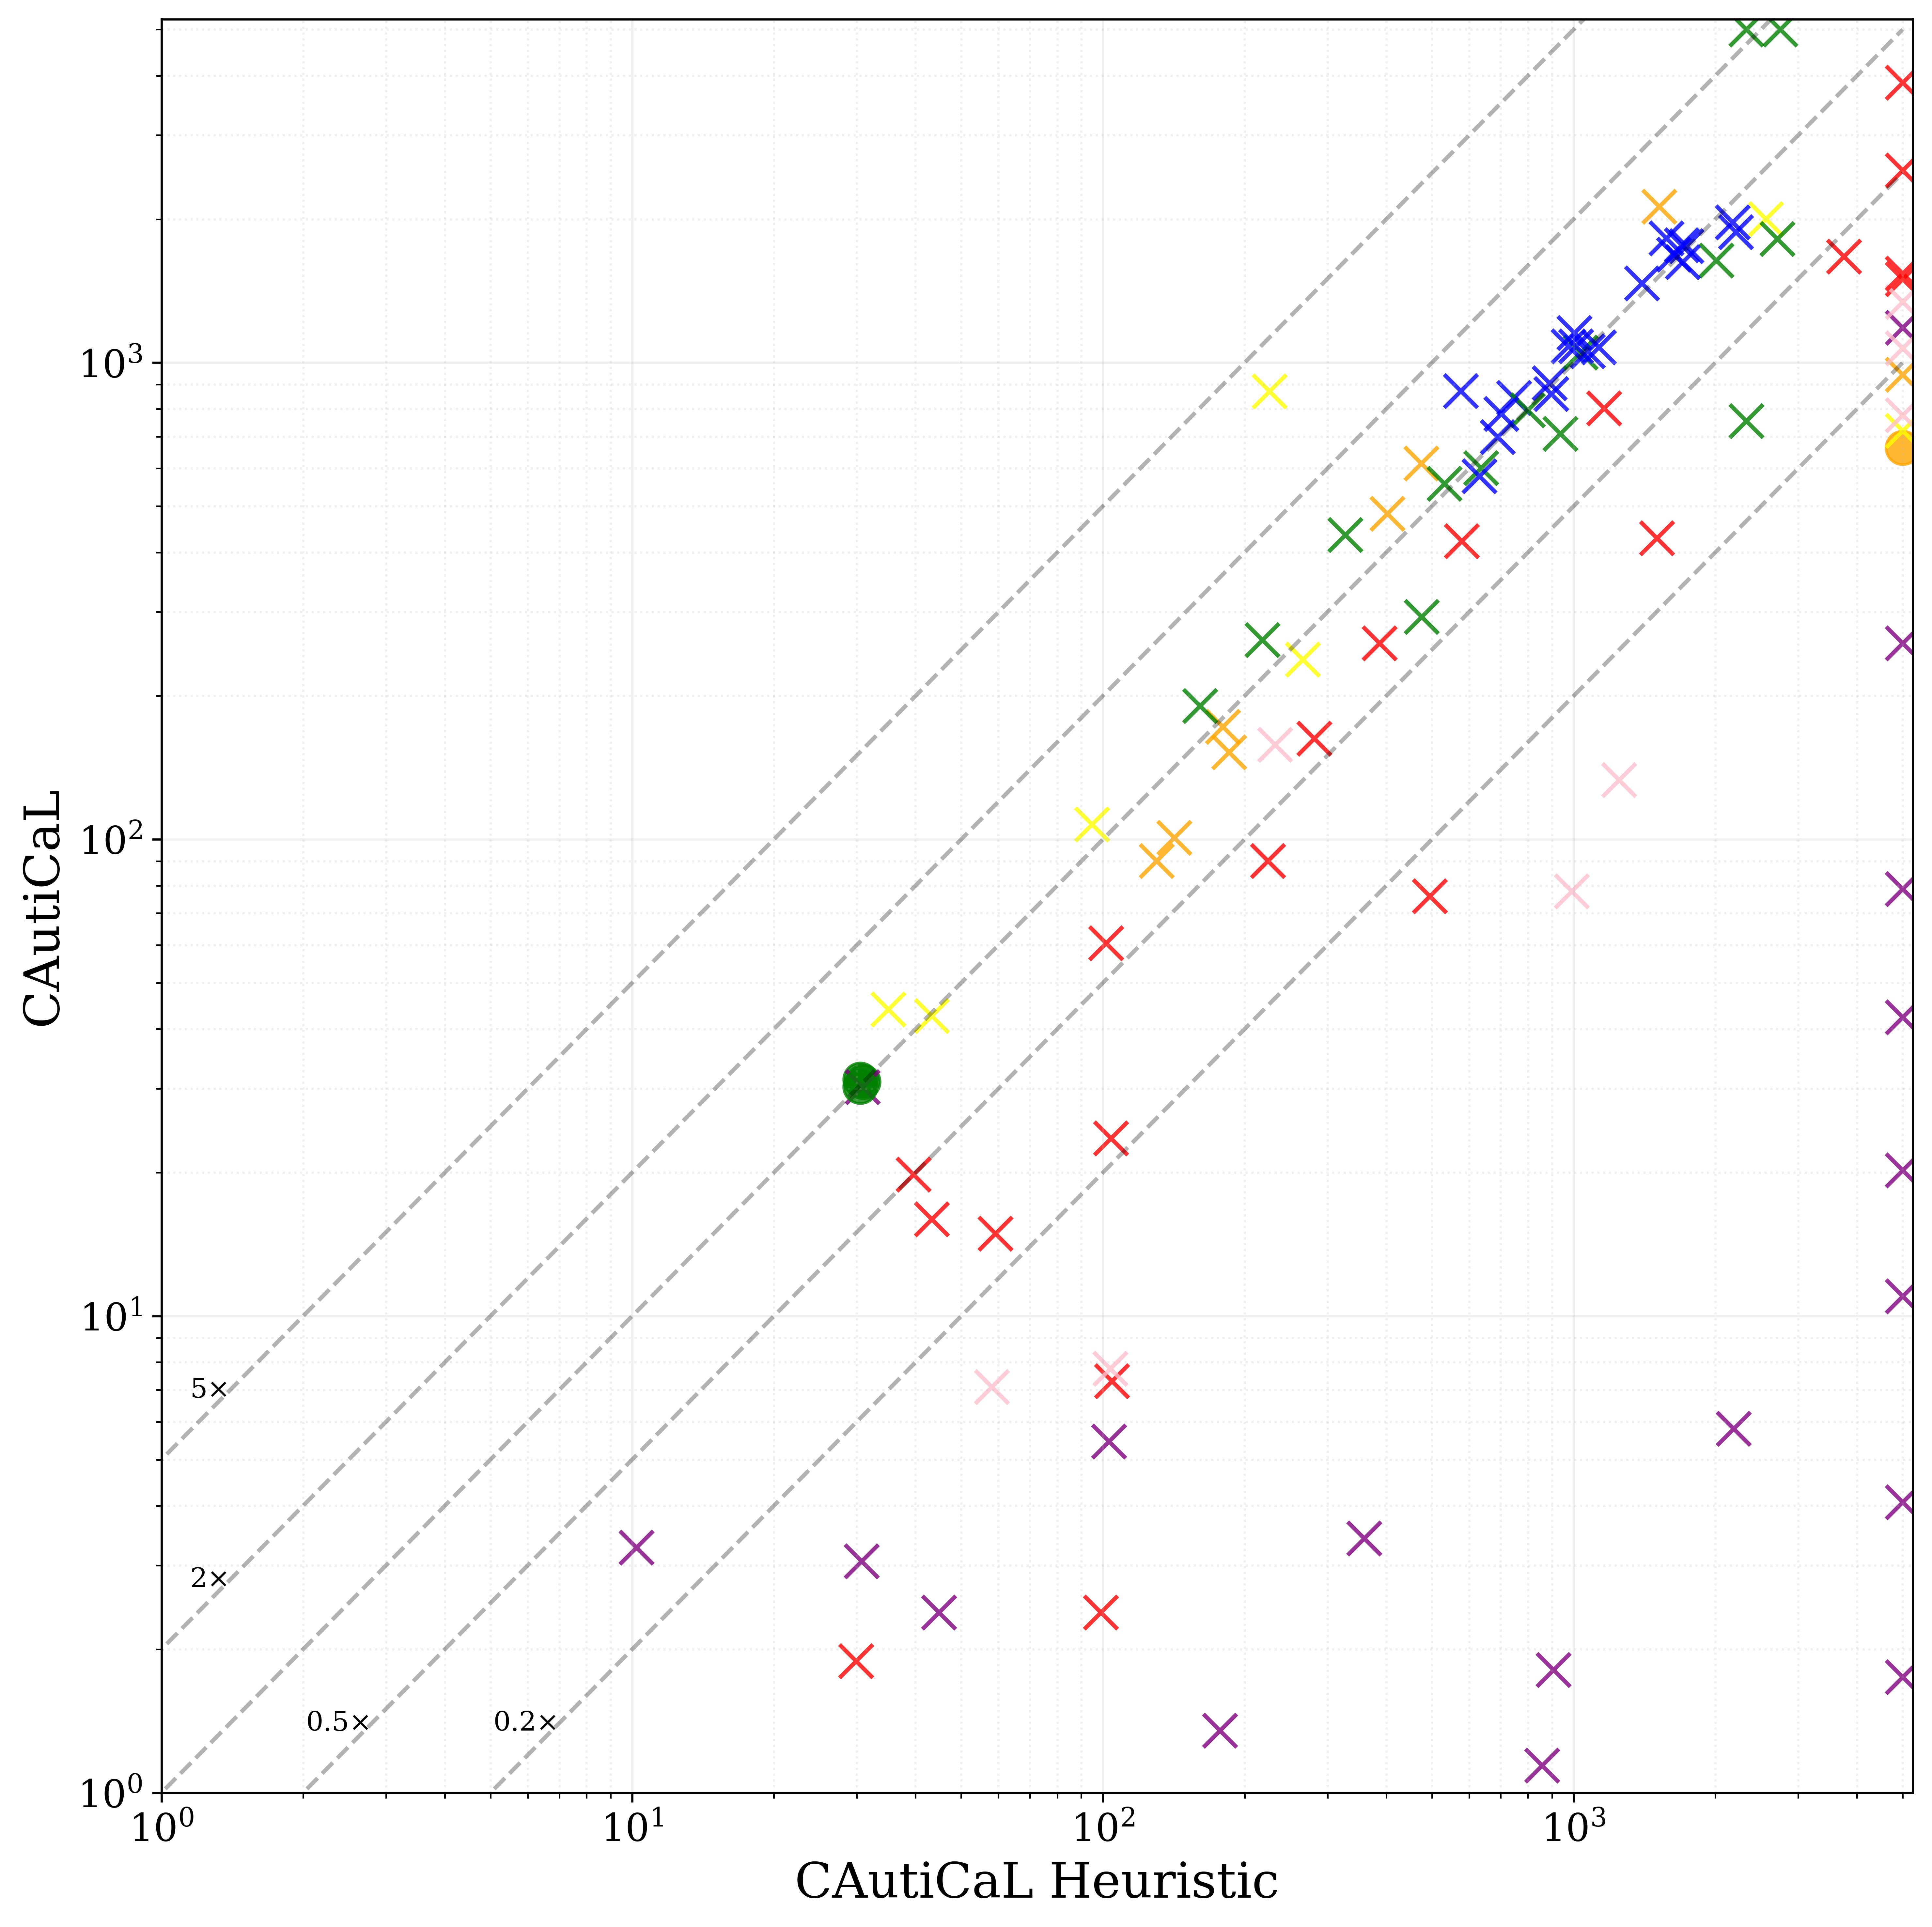
\includegraphics[width=\textwidth]{figs/globaldontfilter_heuristic_comparison.jpg}
        \caption{\tool compared to \tool with \textsf{filter-triv} turned off}
        \label{fig:globaldontfilter}
    \end{subfigure}
    \hfill
    \begin{subfigure}[t]{0.3\textwidth}
        \centering
        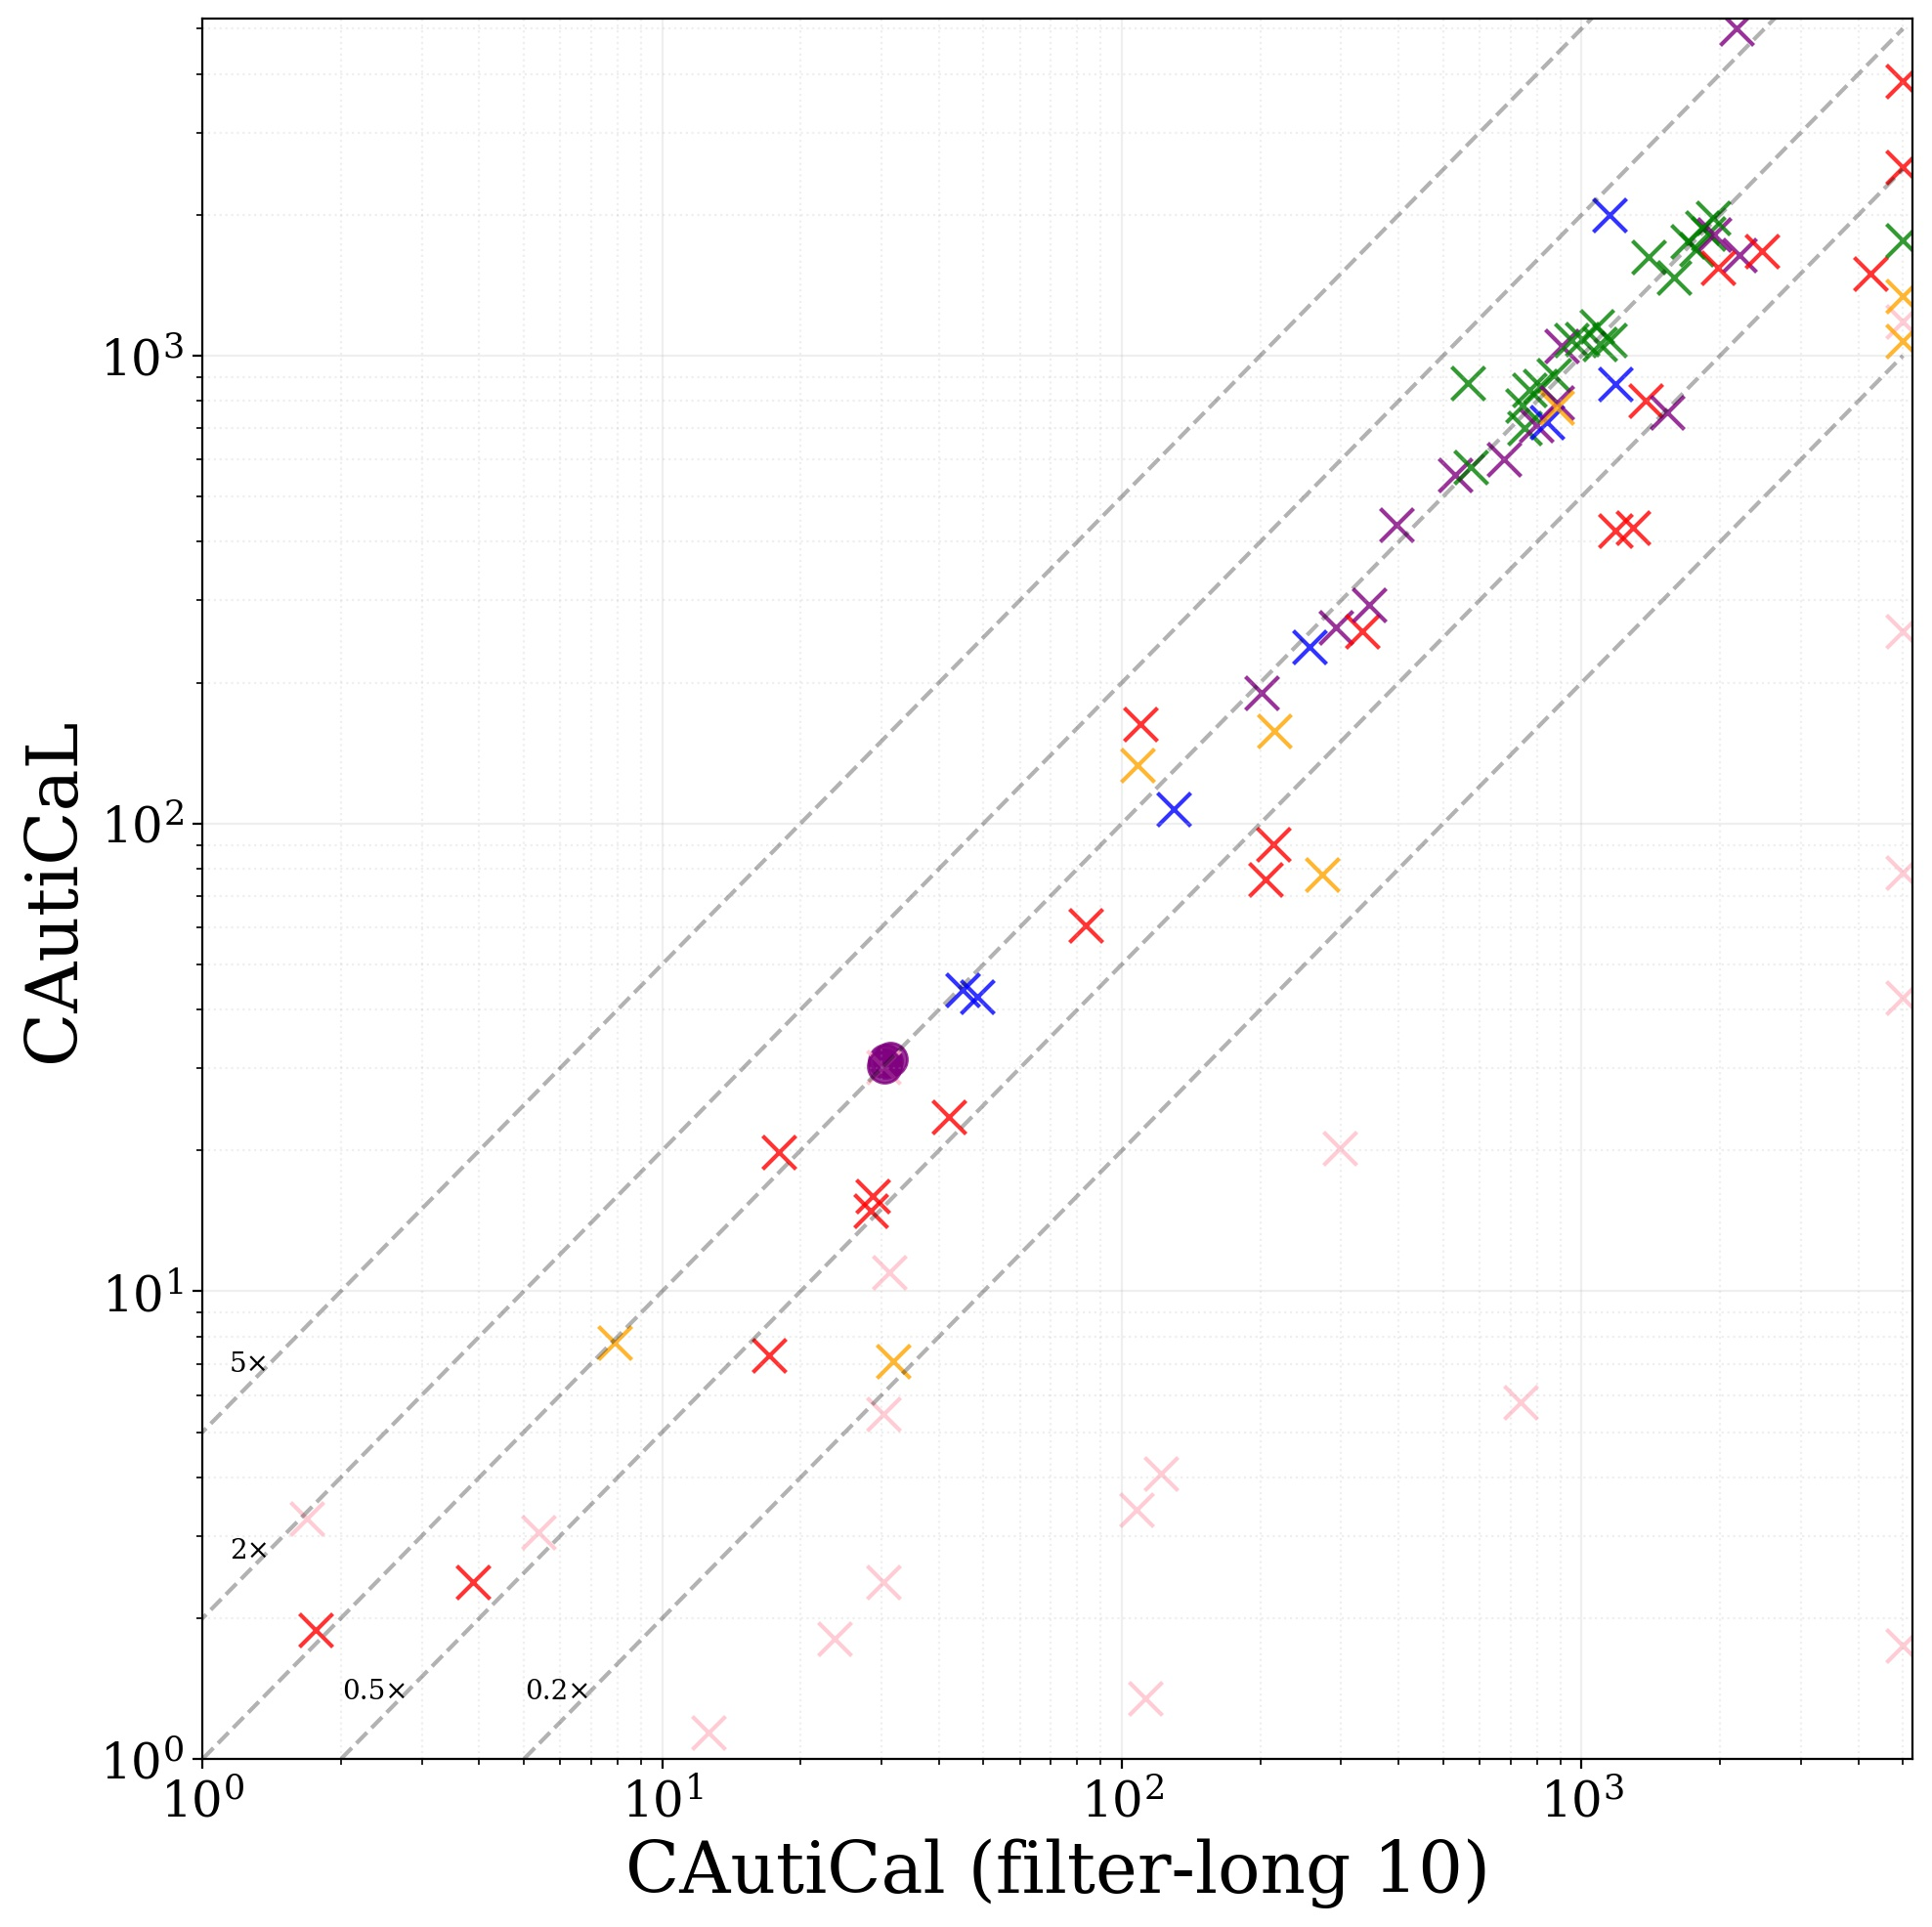
\includegraphics[width=\textwidth]{figs/globalmaxlen_heuristic_comparison.jpg}
        \caption{\tool compared to \tool with \textsf{filter-long} set to $10$}
        \label{fig:global-max-length}
    \end{subfigure} 
    \hfill
    \begin{subfigure}[t]{0.3\textwidth}
        \centering
        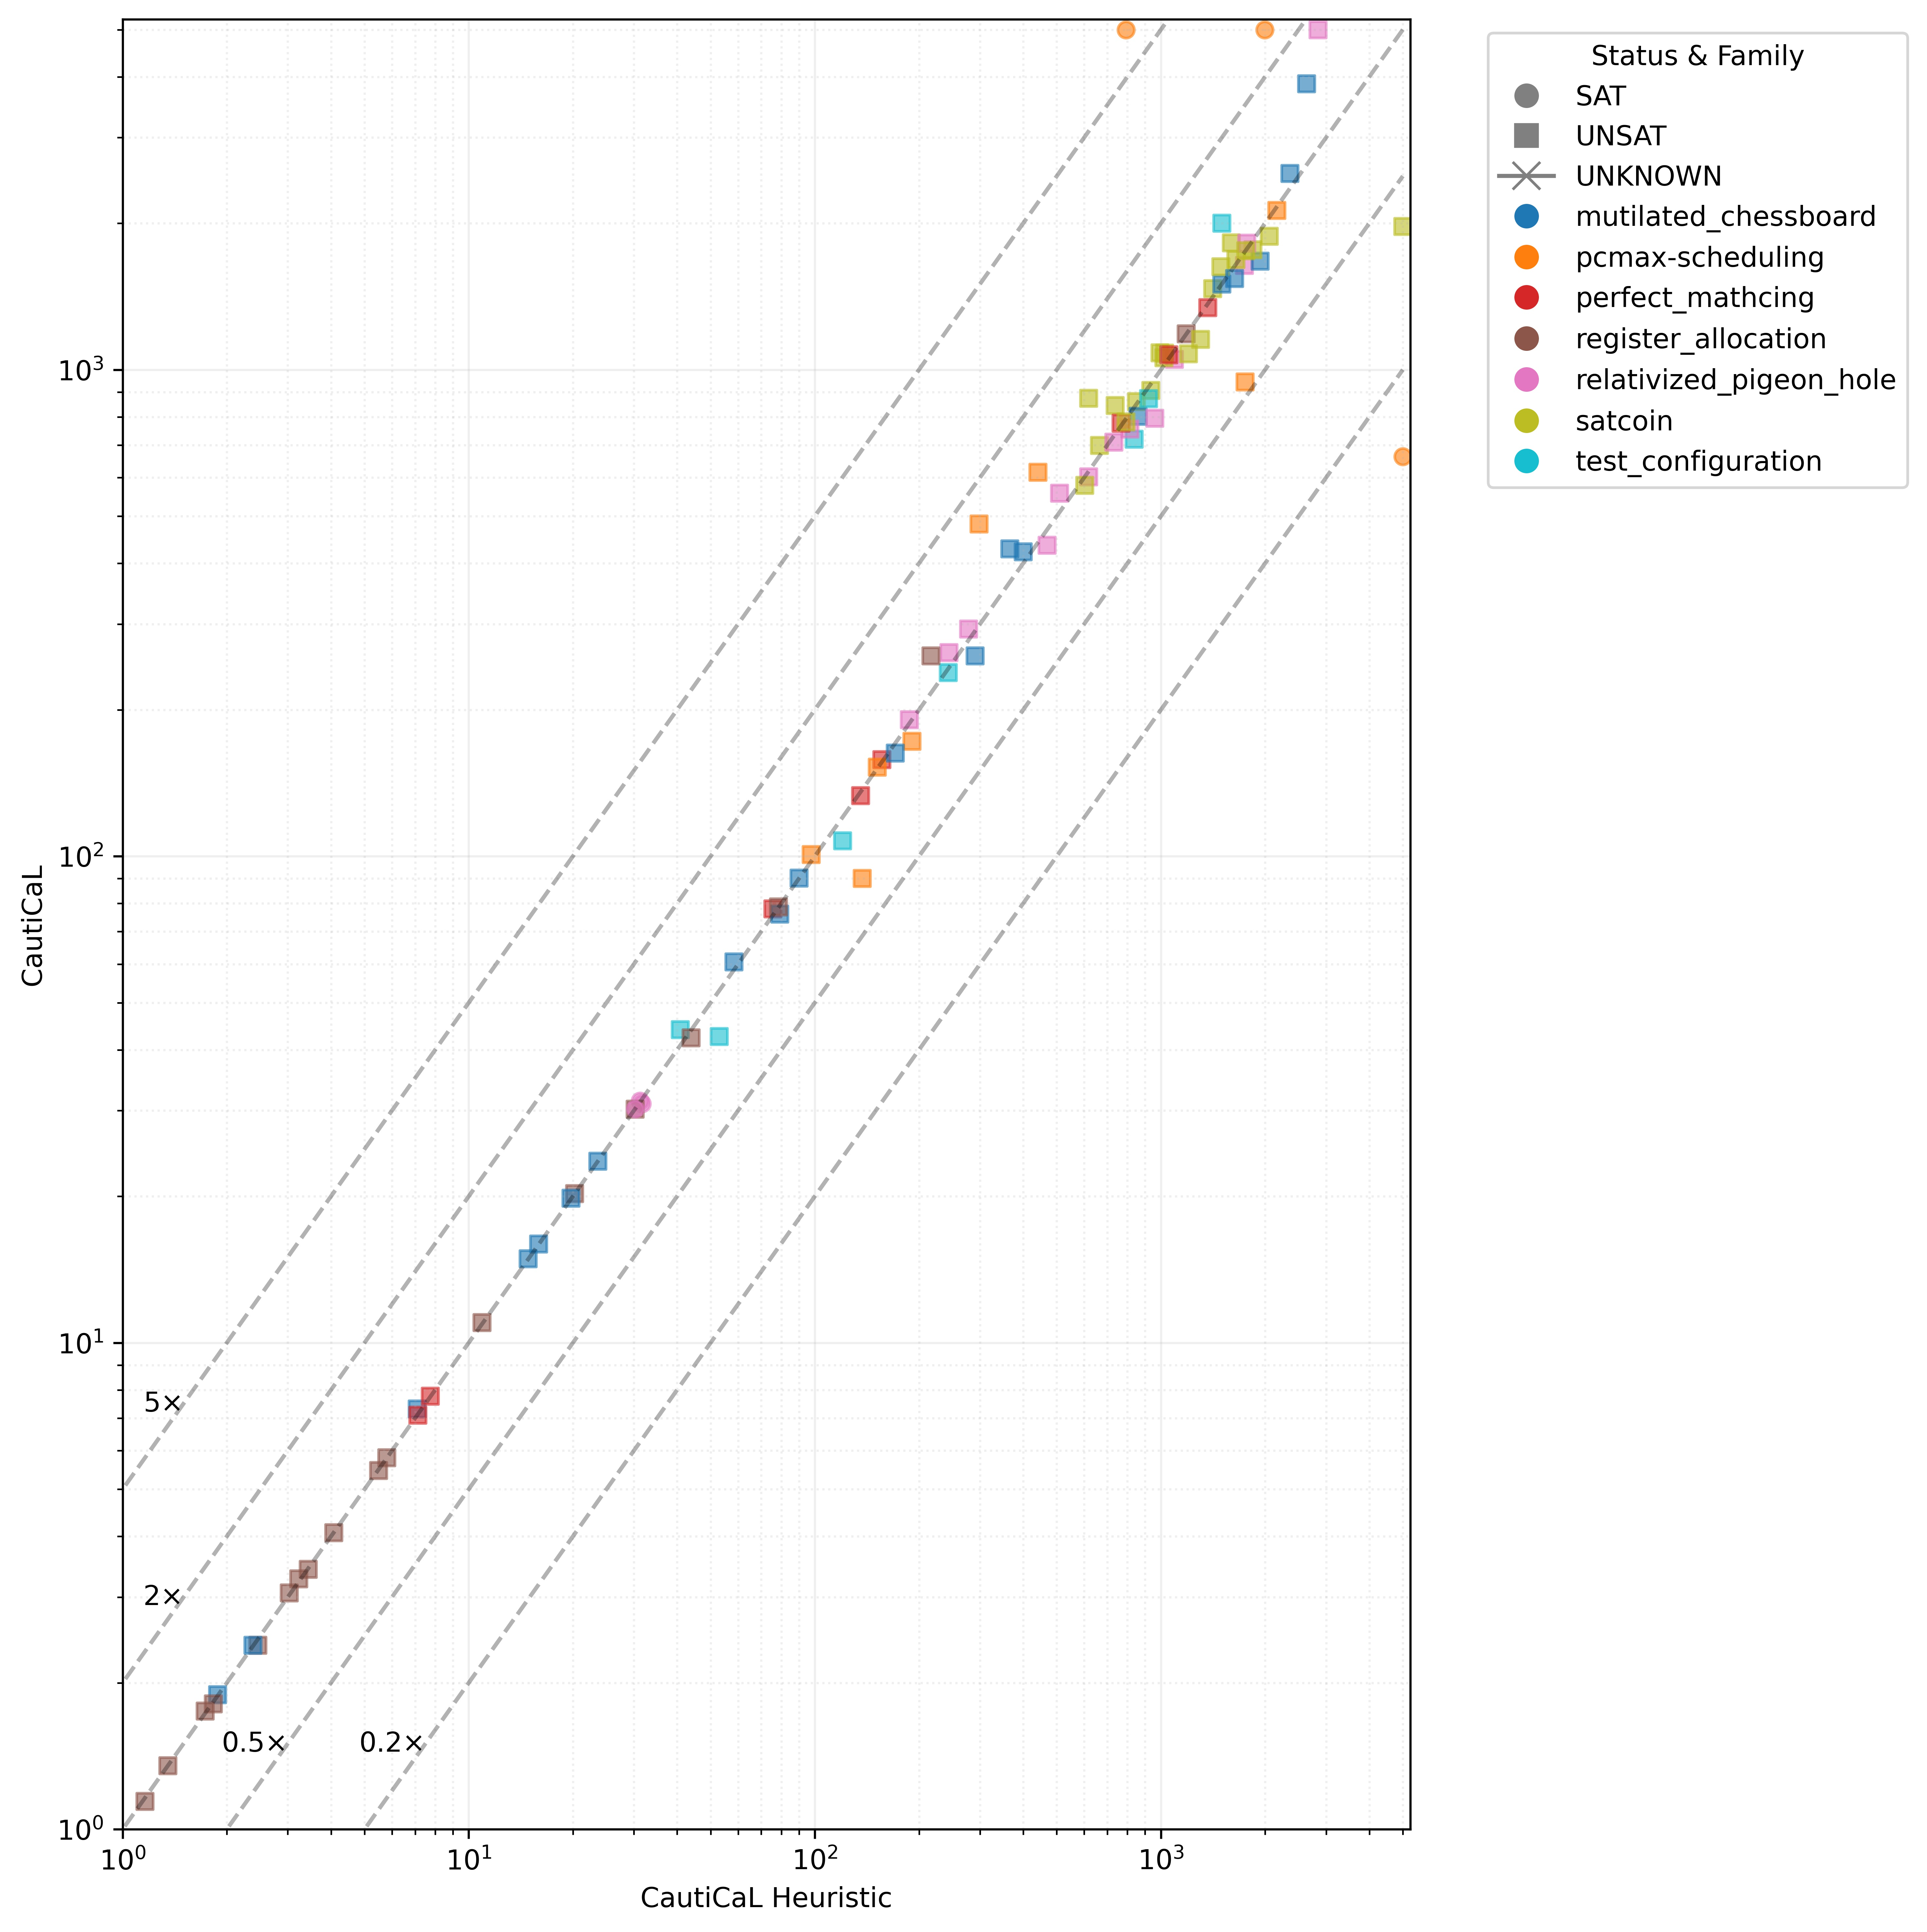
\includegraphics[width=\textwidth]{figs/global_time_lim_heuristic_comparison.jpg}
        \caption{\tool compared to \tool with \textsf{longer-preprocess} set to $100$ seconds}
        \label{fig:global-time-limit}
    \end{subfigure}
    \hfill    
    \begin{subfigure}[t]{0.3\textwidth}
        \centering
        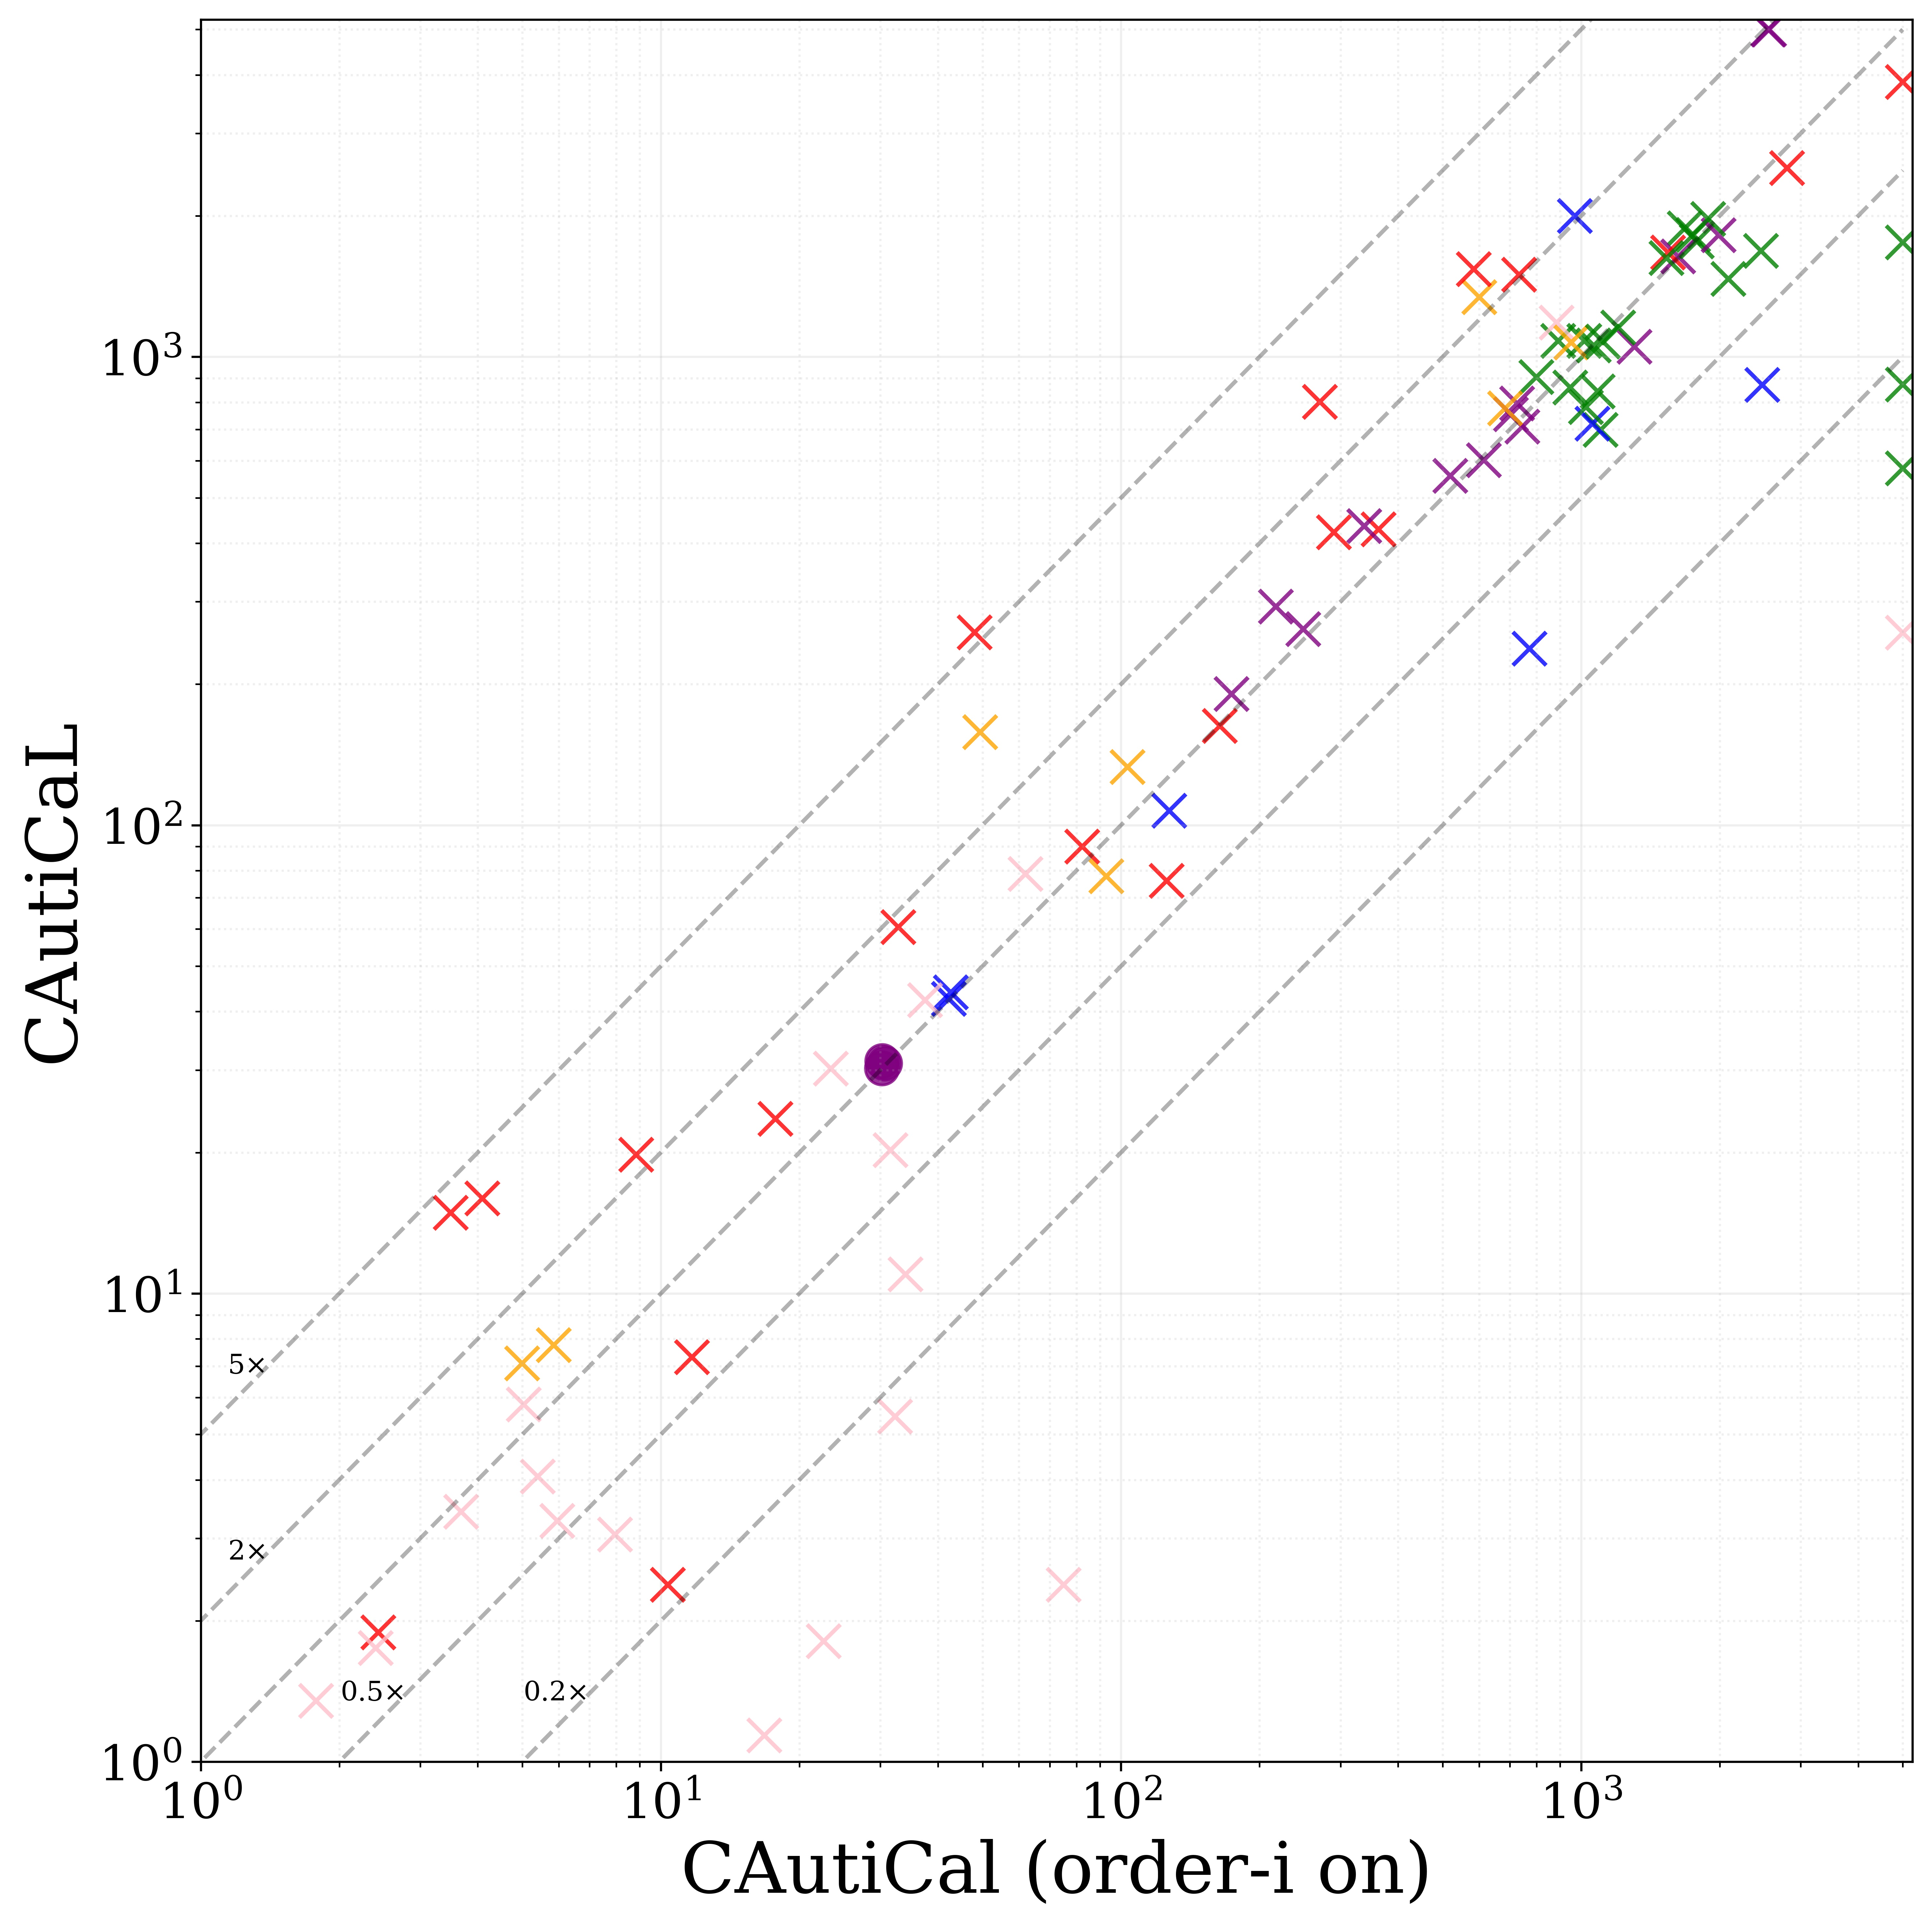
\includegraphics[width=\textwidth]{figs/globalisort_heuristic_comparison.jpg}
        \caption{\tool compared to \tool with \textsf{order-i} turned on}
        \label{fig:global-sort-i}
    \end{subfigure}
    \hfill
    \begin{subfigure}[t]{0.3\textwidth}
        \centering
        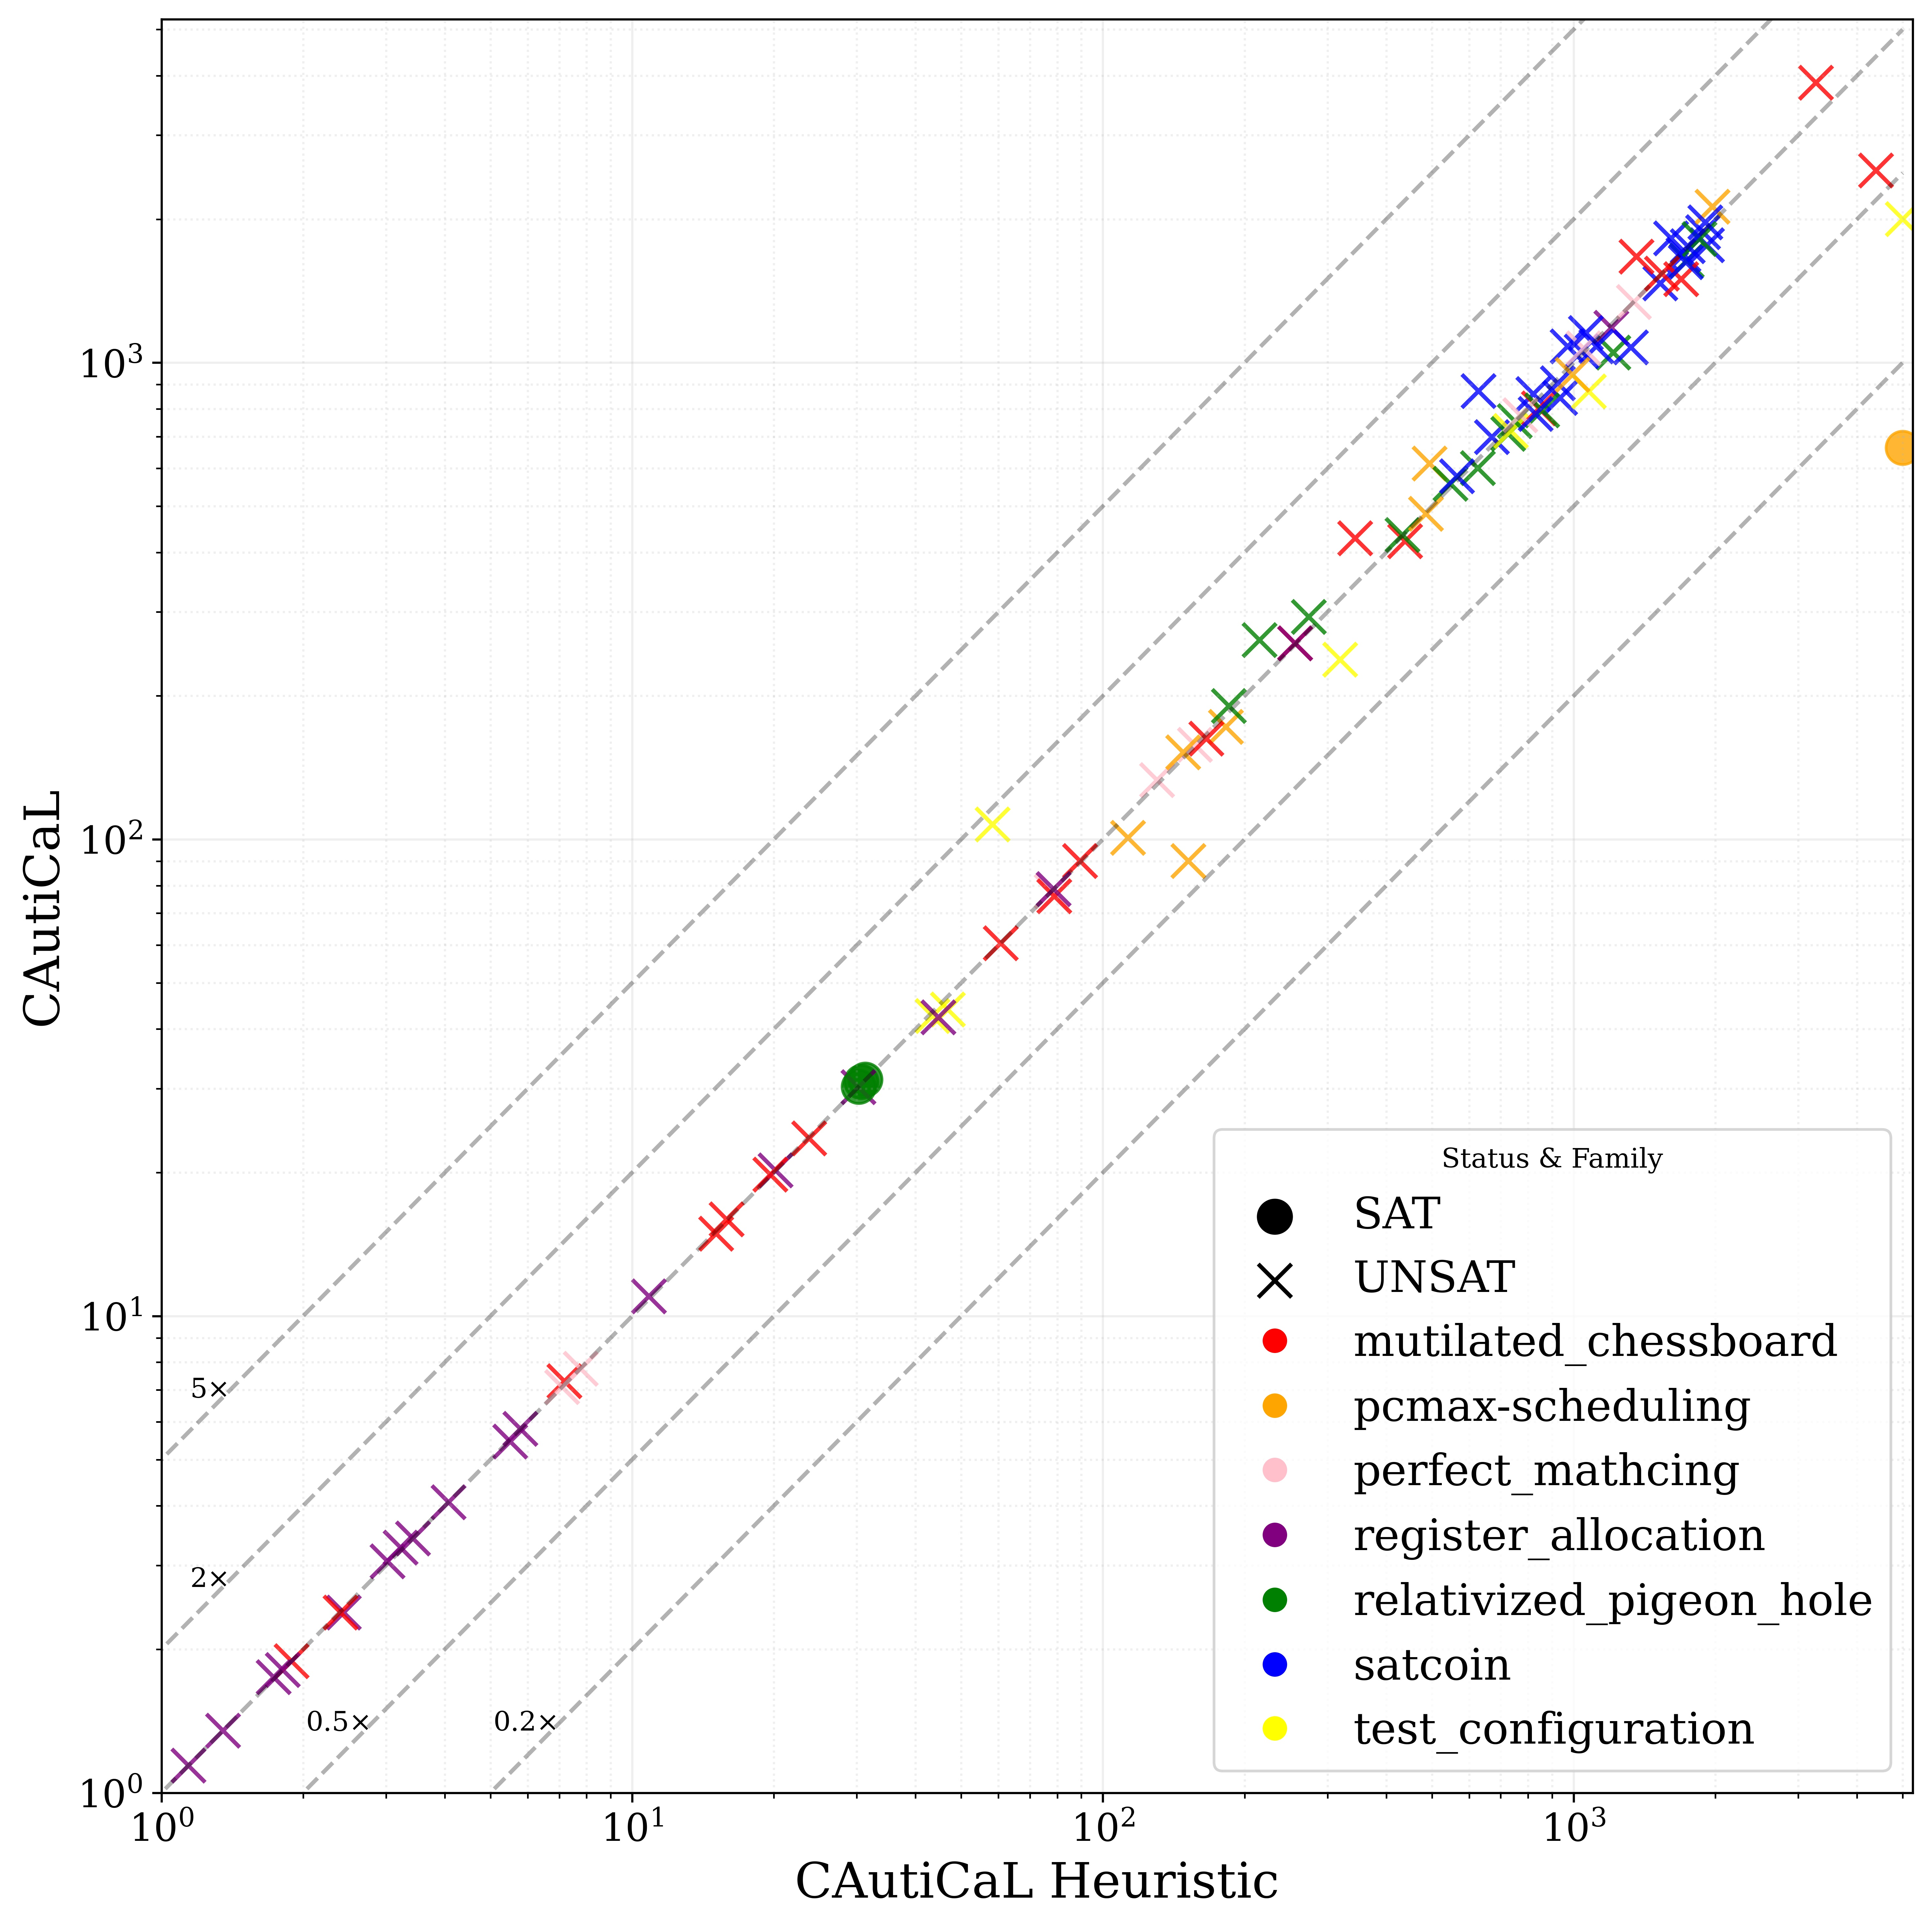
\includegraphics[width=\textwidth]{figs/globaltouch_heuristic_comparison.jpg}
        \caption{\tool compared to \tool with \textsf{select-j} turned on}
        \label{fig:global-touched}
    \end{subfigure}
    \caption{Performance comparison of \tool with other
    solvers}~\label{fig:global-heuristics}
\end{figure*}



\subsection{Heuristics}~\label{app:heuristics}




\autoref{fig:global-heuristics} shows the performance of \tool with different
heuristics (discussed in \autoref{sec:implementation}) turned on and off. We
evaluate on the different benchmark families discussed in
\autoref{subsec:eval-discussion}.

First we consider turning three optimizations off.
\autoref{fig:global-no-shrink} compares \cadical to \cadical with
\textsf{shrink} turned off, i.e. we do not shrink globally blocked clauses.
\autoref{fig:globaldontfilter} compares \cadical to when we turn
\textsf{filter-triv} off, i.e. we do not filter trivial clauses.
\autoref{fig:global-max-length} compares \cadical to when we turn
\textsf{filter-long} to $10$, i.e. we filter out clauses of size $> 10$ (as opposed to $2$ by default).

When we disable any of three optimizations, the performance is significantly
worse, especially on \texttt{perfect-matching}, \texttt{mutilated-chessboard},
and \texttt{register-allocation} benchmarks.

Next, we consider turning three potential ``optimizations'' on.
\autoref{fig:global-time-limit} sets \textsf{longer-preprocess} to 100 seconds (as opposed to 30 seconds by default).
\autoref{fig:global-sort-i} turns on \textsf{order-i}, propagating the first literal $i$ 
ordered by which literals occurs most frequently in the original formula.
Finally, \autoref{fig:global-heuristics} turns on \textsf{select-j}, picking $j$
the second literal by whether it ``touches'' the first literal $i$.

Enabling any of these three ``optimizations'' does not improve performance and in the 
case of \textsf{order-i}, it actually hurts performance.